% Compile with XeLaTeX.
% Executive/technical onboarding deck: project scope and stakeholder decision design.

\documentclass[aspectratio=169,11pt]{beamer}

\usepackage{fontspec}
\setmainfont{DejaVu Sans}
\setsansfont{DejaVu Sans}
\setmonofont{DejaVu Sans Mono}
\usepackage{amsmath,amssymb,booktabs,tabularx,array}
\usepackage{tikz}
\usetikzlibrary{arrows.meta,positioning,fit,calc,shapes.geometric}
\usepackage{hyperref}

\usetheme{default}
\usecolortheme{dove}
\setbeamertemplate{navigation symbols}{}
\setbeamertemplate{blocks}[rounded][shadow=false]
\setbeamersize{text margin left=8mm,text margin right=8mm}
\setbeamertemplate{frametitle}{%
  \nointerlineskip%
  \begin{beamercolorbox}[wd=\paperwidth,ht=1.05cm,dp=.32cm,leftskip=8mm,rightskip=8mm]{frametitle}%
    \usebeamerfont{frametitle}\insertframetitle
  \end{beamercolorbox}%
  \nointerlineskip%
  \begin{beamercolorbox}[wd=\paperwidth,ht=2.5pt,dp=0pt,leftskip=8mm]{frametitle accent}%
    \color{fdorange}\rule{1.7cm}{2.5pt}%
  \end{beamercolorbox}%
  \vspace{.12cm}%
}
\setbeamertemplate{footline}{%
  \leavevmode%
  \hbox{%
    \begin{beamercolorbox}[wd=.78\paperwidth,ht=3ex,dp=1.2ex,leftskip=8mm]{author in head/foot}%
      \scriptsize Financial Distress Data\hspace{.8em}\textcolor{fdorange}{/}\hspace{.8em}Onboarding
    \end{beamercolorbox}%
    \begin{beamercolorbox}[wd=.22\paperwidth,ht=3ex,dp=1.2ex,rightskip=8mm plus 1fil]{date in head/foot}%
      \scriptsize\insertframenumber{} / \inserttotalframenumber
    \end{beamercolorbox}%
  }%
}

\definecolor{fdblue}{HTML}{12355B}
\definecolor{fdteal}{HTML}{087E8B}
\definecolor{fdorange}{HTML}{F28F3B}
\definecolor{fdred}{HTML}{C73E1D}
\definecolor{fdgreen}{HTML}{2A9D8F}
\definecolor{fdgray}{HTML}{F3F5F7}
\definecolor{fdink}{HTML}{1F2933}
\definecolor{fdline}{HTML}{D8E1E8}
\setbeamercolor{structure}{fg=fdblue}
\setbeamercolor{frametitle}{fg=white,bg=fdblue}
\setbeamercolor{frametitle accent}{fg=fdorange,bg=white}
\setbeamercolor{normal text}{fg=fdink,bg=white}
\setbeamercolor{background canvas}{bg=white}
\setbeamercolor{block title}{fg=white,bg=fdteal}
\setbeamercolor{block body}{fg=fdink,bg=fdgray!65}
\setbeamercolor{alertblock title}{fg=white,bg=fdred}
\setbeamercolor{alertblock body}{fg=fdink,bg=fdred!6}
\setbeamercolor{exampleblock title}{fg=white,bg=fdgreen}
\setbeamercolor{exampleblock body}{fg=fdink,bg=fdgreen!7}
\setbeamercolor{author in head/foot}{fg=fdink,bg=fdgray}
\setbeamercolor{date in head/foot}{fg=white,bg=fdblue}
\setbeamerfont{frametitle}{family=\sffamily,size=\Large,series=\bfseries}
\setbeamerfont{block title}{size=\normalsize,series=\bfseries}
\setbeamerfont{title}{family=\sffamily,size=\huge,series=\bfseries}
\setbeamerfont{subtitle}{family=\sffamily,size=\large}
\setbeamertemplate{itemize item}{\color{fdorange}\raisebox{.15ex}{\rule{.55ex}{.55ex}}}
\setbeamertemplate{itemize subitem}{\color{fdteal}\raisebox{.15ex}{\rule{.4ex}{.4ex}}}
\setbeamertemplate{enumerate item}{\color{fdteal}\insertenumlabel.}
\setlength{\parskip}{.18em}

\newcommand{\good}[1]{\textcolor{fdgreen}{\textbf{#1}}}
\newcommand{\warn}[1]{\textcolor{fdorange}{\textbf{#1}}}
\newcommand{\bad}[1]{\textcolor{fdred}{\textbf{#1}}}
\newcommand{\repo}[1]{\texttt{\scriptsize\detokenize{#1}}}

\title{Financial Distress Data}
\subtitle{Stakeholder-centric risk intelligence for financial distress decisions}
\author{Project onboarding briefing}
\institute{Financial Distress Data Engineering System}
\date{10 August 2026}

\begin{document}

\begin{frame}[plain]
  \vfill
  \begin{beamercolorbox}[sep=1em,wd=\textwidth]{frametitle}
    {\usebeamerfont{title}\inserttitle\par}
    \vspace{.35em}
    {\usebeamerfont{subtitle}\insertsubtitle\par}
  \end{beamercolorbox}
  \vspace{1em}
  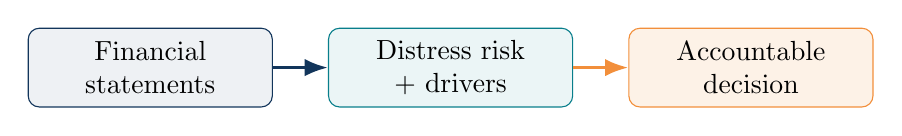
\begin{tikzpicture}[node distance=7mm,>=Latex]
    \node[draw=fdblue,fill=fdblue!7,rounded corners,minimum width=3.1cm,minimum height=1cm,align=center] (data) {Financial\\statements};
    \node[draw=fdteal,fill=fdteal!8,rounded corners,minimum width=3.1cm,minimum height=1cm,align=center,right=of data] (risk) {Distress risk\\+ drivers};
    \node[draw=fdorange,fill=fdorange!12,rounded corners,minimum width=3.1cm,minimum height=1cm,align=center,right=of risk] (decision) {Accountable\\decision};
    \draw[->,very thick,fdblue] (data) -- (risk);
    \draw[->,very thick,fdorange] (risk) -- (decision);
  \end{tikzpicture}
  \vfill
  \centering\small\textcolor{fdink!70}{Trọng tâm: cùng một risk output, nhưng mỗi nhóm sử dụng có mục tiêu, ngưỡng và workflow khác nhau.}
\end{frame}

\begin{frame}{1. Mục tiêu và phạm vi hệ thống}
  \small
  \begin{columns}[T,totalwidth=\textwidth]
    \column{.47\textwidth}
      \begin{block}{Mục tiêu sản phẩm}
        Xây dựng nền tảng dữ liệu hỗ trợ phát hiện sớm nguy cơ financial distress của doanh nghiệp, bảo đảm kết quả có thể truy xuất nguồn gốc và sử dụng trong quy trình ra quyết định.
      \end{block}
      \begin{exampleblock}{Giá trị cung cấp}
        Chuẩn hóa dữ liệu phân tán thành risk score/label, risk drivers, xu hướng và evidence theo từng thời điểm quan sát.
      \end{exampleblock}
    \column{.47\textwidth}
      \begin{block}{Phạm vi hiện tại}
        \begin{itemize}
          \item Ingestion và canonical data contracts.
          \item Data quality, deduplication và time semantics.
          \item Feature/risk output phục vụ downstream consumers.
          \item Foundation local-first; live source integration là bước mở rộng.
        \end{itemize}
      \end{block}
      \centering\scriptsize\warn{Verified foundation không đồng nghĩa live production integration.}
  \end{columns}
\end{frame}

\begin{frame}{2. Chuỗi giá trị dữ liệu và decision output}
  \centering
  \begin{tikzpicture}[>=Latex,node distance=7mm,scale=.86,transform shape]
    \tikzset{stage/.style={draw=fdline,fill=fdgray,rounded corners,minimum width=2.15cm,minimum height=1.05cm,align=center,font=\small}, arrow/.style={->,very thick,fdblue}}
    \node[stage] (source) {Nguồn dữ liệu\\financial / market};
    \node[stage,right=of source] (quality) {Chuẩn hóa\\và DQ};
    \node[stage,right=of quality] (feature) {Feature\\theo thời điểm};
    \node[stage,right=of feature,fill=fdteal!10,draw=fdteal] (model) {Risk score\\+ drivers};
    \node[stage,right=of model,fill=fdorange!12,draw=fdorange] (decision) {Decision\\workflow};
    \draw[arrow] (source) -- (quality);
    \draw[arrow] (quality) -- (feature);
    \draw[arrow] (feature) -- (model);
    \draw[arrow,fdorange] (model) -- (decision);
  \end{tikzpicture}
  \vspace{.8em}
  \begin{columns}[T,totalwidth=\textwidth]
    \column{.31\textwidth}\centering\scriptsize\textbf{Data contract}\\Source + schema + time + key.
    \column{.31\textwidth}\centering\scriptsize\textbf{Model contract}\\Score/label + driver + threshold.
    \column{.31\textwidth}\centering\scriptsize\textbf{Decision contract}\\Người nhận + hành động + escalation.
  \end{columns}
\end{frame}

\begin{frame}{3. Nguyên tắc thiết kế: stakeholder-centric risk intelligence}
  \begin{columns}[T,totalwidth=\textwidth]
    \column{.44\textwidth}
      \begin{block}{Model-centric view}
        \begin{itemize}
          \item Tập trung vào accuracy, AUC hoặc classification label.
          \item Output kết thúc ở dashboard/API.
          \item Cùng một threshold cho mọi nhóm sử dụng.
        \end{itemize}
      \end{block}
    \column{.50\textwidth}
      \begin{exampleblock}{Stakeholder-centric view}
        \begin{enumerate}
          \item Xác định stakeholder và quyết định cần hỗ trợ.
          \item Định nghĩa cost của false positive/false negative.
          \item Chọn output, metric, threshold và explainability phù hợp.
          \item Đưa kết quả vào workflow và đo business impact.
        \end{enumerate}
      \end{exampleblock}
  \end{columns}
  \vfill
  \centering\large Stakeholder \textrightarrow{} decision \textrightarrow{} cost of error \textrightarrow{} output \textrightarrow{} workflow
\end{frame}

\begin{frame}{4. Một risk score, ba quyết định kinh doanh}
  \begin{alertblock}{Tình huống minh họa}
    Doanh nghiệp A có \bad{distress risk = 82\%}. Con số này chỉ tạo giá trị khi được diễn giải trong đúng bối cảnh sử dụng.
  \end{alertblock}
  \vspace{.4em}
  \begin{columns}[T,totalwidth=\textwidth]
    \column{.31\textwidth}
      \centering\textcolor{fdblue}{\Large\textbf{Lender}}\\
      \vspace{.3em}\small Quyết định cấp tín dụng, hạn mức và tái tục.
    \column{.31\textwidth}
      \centering\textcolor{fdteal}{\Large\textbf{Investor}}\\
      \vspace{.3em}\small Quyết định nghiên cứu, theo dõi hoặc tái phân bổ danh mục.
    \column{.31\textwidth}
      \centering\textcolor{fdorange}{\Large\textbf{Management}}\\
      \vspace{.3em}\small Quyết định khắc phục dòng tiền, nợ, chi phí và vốn.
  \end{columns}
  \vfill
  \centering\small\textcolor{fdink!70}{Không có một cách diễn giải duy nhất cho cùng một model output.}
\end{frame}

\begin{frame}{5. Ngân hàng — Tín dụng và giám sát rủi ro}
  \scriptsize
  \begin{columns}[T,totalwidth=\textwidth]
    \column{.39\textwidth}
      \begin{block}{Decision objective}
        Đánh giá khả năng doanh nghiệp duy trì nghĩa vụ nợ trong kỳ cấp tín dụng, điều chỉnh hạn mức hoặc tái tục.
      \end{block}
      \begin{block}{Evidence required}
        \begin{itemize}
          \item Debt ratio, current ratio và interest coverage.
          \item Operating cash flow, profitability và leverage trend.
          \item Collateral, exposure, repayment history và data freshness.
        \end{itemize}
      \end{block}
    \column{.55\textwidth}
      \begin{exampleblock}{Decision output}
        Risk score/label đi kèm driver, as-of date, provenance và lý do escalation; không phải quyết định tự động.
      \end{exampleblock}
      \begin{alertblock}{Human action}
        Standard review \textrightarrow{} enhanced due diligence \textrightarrow{} bảo đảm/giảm hạn mức \textrightarrow{} phê duyệt có điều kiện hoặc từ chối.
      \end{alertblock}
  \end{columns}
\end{frame}

\begin{frame}{6. Ngân hàng — Chính sách ngưỡng và quy trình escalation}
  \scriptsize
  \begin{columns}[T,totalwidth=\textwidth]
    \column{.48\textwidth}
      \begin{block}{Cost-sensitive evaluation}
        Bỏ sót một doanh nghiệp có distress có thể gây tổn thất lớn hơn chi phí review nhầm một hồ sơ tốt.
        \[
          \mathrm{Recall}=\frac{TP}{TP+FN}
          \qquad
          \mathrm{Precision}=\frac{TP}{TP+FP}
        \]
      \end{block}
      \begin{exampleblock}{Threshold không chọn theo accuracy đơn lẻ}
        \scriptsize
        \[
          \begin{aligned}
            \mathrm{Expected\ Loss}(\tau)&=C_{FN}FN(\tau)+C_{FP}FP(\tau)\\
            &\quad+C_{review}N_{review}(\tau)
          \end{aligned}
        \]
      \end{exampleblock}
    \column{.46\textwidth}
      \begin{block}{Operational workflow}
        \begin{enumerate}
          \item Score vượt threshold: đưa vào enhanced review.
          \item Kiểm tra driver, evidence và dữ liệu mới nhất.
          \item Quyết định limit/collateral/approval và ghi audit trail.
          \item Theo dõi lại ở kỳ tiếp theo hoặc trước renewal.
        \end{enumerate}
      \end{block}
      \centering\scriptsize\warn{Threshold cần hiệu chỉnh theo portfolio, risk appetite và năng lực review.}
  \end{columns}
\end{frame}

\begin{frame}[shrink=8]{7. Nhà đầu tư — Nghiên cứu và giám sát danh mục}
  \small
  \begin{columns}[T,totalwidth=\textwidth]
    \column{.41\textwidth}
      \begin{block}{Decision objective}
        Đánh giá sức khỏe tài chính đang cải thiện hay suy giảm để ưu tiên research, theo dõi holding hoặc tái phân bổ danh mục.
      \end{block}
      \begin{exampleblock}{Risk trajectory}
        \scriptsize
        \centering
        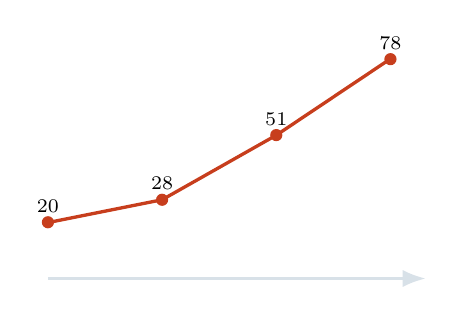
\begin{tikzpicture}[>=Latex]
          \draw[fdline,very thick,->] (0,0) -- (4.8,0);
          \foreach \x/\v in {0/20,1.45/28,2.9/51,4.35/78}{
            \fill[fdred] (\x,{\v/28}) circle (2.2pt);
            \node[above,font=\scriptsize] at (\x,{\v/28}) {\v};
          }
          \draw[fdred,very thick] (0,.71) -- (1.45,1) -- (2.9,1.82) -- (4.35,2.79);
        \end{tikzpicture}
      \end{exampleblock}
    \column{.54\textwidth}
      \begin{block}{Information required}
        \scriptsize
        \begin{itemize}
          \item Trend, change-point và mức độ bền vững của tín hiệu.
          \item Risk drivers: leverage, cash flow, interest coverage, profitability.
          \item Peer/context, market signal và confidence/provenance.
        \end{itemize}
      \end{block}
      \begin{alertblock}{Decision boundary}
        \scriptsize
        Risk intelligence hỗ trợ research và portfolio review; không thay thế investment thesis và không tự động phát sinh lệnh buy/sell.
      \end{alertblock}
  \end{columns}
\end{frame}

\begin{frame}{8. Nhà đầu tư — Explainability và chất lượng tín hiệu}
  \scriptsize
  \begin{columns}[T,totalwidth=\textwidth]
    \column{.46\textwidth}
      \begin{exampleblock}{Từ label đến explanation}
        \textbf{High risk = 78\%} cần được phân rã thành các yếu tố đóng góp:
        \begin{itemize}
          \item Debt ratio tăng: contribution dương.
          \item Operating cash flow suy yếu.
          \item Interest coverage và profitability giảm.
        \end{itemize}
        Explanation giúp analyst kiểm tra tính hợp lý, không biến correlation thành causal claim.
      \end{exampleblock}
    \column{.46\textwidth}
      \begin{block}{Metrics phù hợp với research}
        \begin{itemize}
          \item Alert precision và tỷ lệ tín hiệu hữu ích.
          \item Lead time trước khi distress được quan sát.
          \item Stability của trend và consistency của driver.
          \item Coverage theo sector, size và reporting cadence.
        \end{itemize}
      \end{block}
  \end{columns}
\end{frame}

\begin{frame}{9. Ban điều hành — Early warning và remediation}
  \small
  \begin{columns}[T,totalwidth=\textwidth]
    \column{.39\textwidth}
      \begin{alertblock}{Decision objective}
        Nhận diện sớm yếu tố có thể đẩy doanh nghiệp vào distress và ưu tiên biện pháp khắc phục.
      \end{alertblock}
      \begin{block}{Risk trajectory}
        \centering\large 18\% \textrightarrow{} 25\% \textrightarrow{} 46\% \textrightarrow{} \bad{71\%}
        \par\scriptsize Xu hướng tăng liên tục cần chuyển thành operational alert.
      \end{block}
    \column{.55\textwidth}
      \begin{exampleblock}{Risk drivers cần chuyển thành owner/action}
        \scriptsize
        \begin{tabularx}{\linewidth}{>{\bfseries}p{.33\linewidth} X}
          Driver & Hướng xử lý\\\midrule
          Debt tăng & Rà soát lịch trả nợ, tái cấu trúc, giảm leverage.\\
          Cash flow yếu & Theo dõi liquidity, công nợ và working capital.\\
          Chi phí tăng & Phân rã cost driver, gán owner và deadline.\\
          Vốn mỏng & Xem xét equity, retained earnings và capital plan.\\
        \end{tabularx}
      \end{exampleblock}
  \end{columns}
\end{frame}

\begin{frame}{10. Ban điều hành — Quy trình từ driver đến action}
  \begin{columns}[T,totalwidth=\textwidth]
    \column{.48\textwidth}
      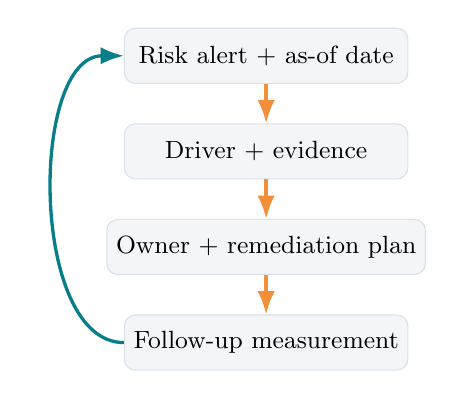
\begin{tikzpicture}[>=Latex,node distance=5mm]
        \tikzset{loop/.style={draw=fdline,fill=fdgray,rounded corners,minimum width=3.6cm,minimum height=.7cm,align=center,font=\small}}
        \node[loop] (alert) {Risk alert + as-of date};
        \node[loop,below=of alert] (driver) {Driver + evidence};
        \node[loop,below=of driver] (owner) {Owner + remediation plan};
        \node[loop,below=of owner] (monitor) {Follow-up measurement};
        \draw[->,very thick,fdorange] (alert) -- (driver);
        \draw[->,very thick,fdorange] (driver) -- (owner);
        \draw[->,very thick,fdorange] (owner) -- (monitor);
        \draw[->,very thick,fdteal] (monitor.west) .. controls ++(-1.2,0) and ++(-1.2,0) .. (alert.west);
      \end{tikzpicture}
    \column{.45\textwidth}
      \begin{block}{Metrics của workflow}
        \begin{itemize}
          \item Lead time trước khi distress xảy ra.
          \item Time-to-acknowledge và time-to-mitigate.
          \item Tỷ lệ alert có owner và remediation plan.
          \item Residual risk sau mỗi kỳ theo dõi.
        \end{itemize}
      \end{block}
      \centering\small\good{Model thành công khi cảnh báo dẫn đến hành động có thể kiểm chứng.}
  \end{columns}
\end{frame}

\begin{frame}{11. So sánh ba decision products}
  \scriptsize
  \renewcommand{\arraystretch}{1.45}
  \begin{tabularx}{\textwidth}{>{\bfseries}p{.18\textwidth} p{.22\textwidth} X p{.24\textwidth}}
    User group & Decision objective & Priority output & Success measure\\\midrule
    Lender & Underwriting, limit và renewal & Score, driver, exposure, collateral context, escalation & Recall/precision theo cost; review efficiency\\
    Investor & Research, monitoring và portfolio review & Trend, change-point, explanation, peer/context, confidence & Alert precision, lead time, signal stability\\
    Management & Early warning và remediation & Driver, owner, deadline, action status, residual risk & Time-to-action, closure rate, residual-risk reduction\\
  \end{tabularx}
  \vfill
  \begin{block}{Kết luận thiết kế}
    Một model backbone có thể dùng chung; decision product, threshold policy, explanation và workflow phải được thiết kế theo từng nhóm sử dụng.
  \end{block}
\end{frame}

\begin{frame}{12. Shared data contract và stakeholder-specific view}
  \centering
  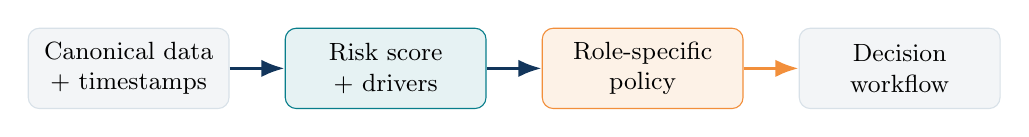
\begin{tikzpicture}[>=Latex,node distance=7mm]
    \tikzset{box/.style={draw=fdline,fill=fdgray,rounded corners,minimum width=2.55cm,minimum height=1.02cm,align=center,font=\small}}
    \node[box] (data) {Canonical data\\+ timestamps};
    \node[box,right=of data,fill=fdteal!10,draw=fdteal] (risk) {Risk score\\+ drivers};
    \node[box,right=of risk,fill=fdorange!12,draw=fdorange] (policy) {Role-specific\\policy};
    \node[box,right=of policy] (workflow) {Decision\\workflow};
    \draw[->,very thick,fdblue] (data) -- (risk);
    \draw[->,very thick,fdblue] (risk) -- (policy);
    \draw[->,very thick,fdorange] (policy) -- (workflow);
  \end{tikzpicture}
  \vspace{.7em}
  \begin{columns}[T,totalwidth=\textwidth]
    \column{.31\textwidth}\centering\textbf{Shared layer}\par\small Entity, metric, period, source, effective time, DQ và lineage.
    \column{.31\textwidth}\centering\textbf{Role layer}\par\small Decision objective, threshold, evidence và explanation theo stakeholder.
    \column{.31\textwidth}\centering\textbf{Governance layer}\par\small Human review, audit trail, access control, feedback và conflict handling.
  \end{columns}
\end{frame}

\begin{frame}{13. Chuyển đổi nguồn: API và stakeholder research}
  \begin{alertblock}{Định hướng kiến trúc}
    Stakeholder research là lớp bổ sung context và judgement; không thay thế toàn bộ nguồn numeric facts có cấu trúc.
  \end{alertblock}
  \vspace{.2em}
  \scriptsize
  \begin{enumerate}
    \item \textbf{Bảo toàn canonical contract}: business key, effective time, schema, DQ và lineage.
    \item \textbf{Thêm research adapter}: document, observation, author/role, confidence, evidence và review status.
    \item \textbf{Chuẩn hóa có kiểm soát}: lưu raw text, normalized observation và mapping vào entity/metric/period.
    \item \textbf{Xử lý disagreement}: giữ conflict history; không âm thầm ghi đè API facts bằng judgement.
    \item \textbf{Shadow run trước cutover}: đo coverage, freshness, conflict rate và decision usefulness.
  \end{enumerate}
  \centering\small\warn{Mục tiêu là mở rộng bằng adapter và governance, không phá vỡ downstream contract.}
\end{frame}

\begin{frame}{14. Migration governance và acceptance criteria}
  \scriptsize
  \renewcommand{\arraystretch}{1.45}
  \begin{tabularx}{\textwidth}{>{\bfseries}p{.23\textwidth} X p{.28\textwidth}}
    Control point & Cách kiểm chứng & Điều kiện để tiến tới cutover\\\midrule
    Contract compatibility & Schema, key, timestamp và downstream tests & Không phá vỡ public contract hiện tại\\
    Data quality & Completeness, validity, duplication và freshness & Đạt ngưỡng DQ theo từng source/role\\
    Source agreement & So sánh API facts, research observations và conflict history & Conflict được phân loại, review và truy xuất được\\
    Decision usefulness & User acceptance, alert precision, lead time, time-to-action & Có bằng chứng workflow tạo ra giá trị\\
    Rollback safety & Snapshot/API fallback và audit trail & Cutover có thể đảo chiều không mất provenance\\
  \end{tabularx}
  \vfill
  \centering\small\textcolor{fdink!70}{Phân biệt rõ ba trạng thái: verified behavior, proposed design và production evidence.}
\end{frame}

\begin{frame}{15. Kết luận — Từ prediction đến decision có trách nhiệm}
  \vfill
  \begin{block}{Thông điệp kết thúc}
    Financial Distress Data không chỉ tạo ra một risk score. Hệ thống tạo ra nền tảng dữ liệu để mỗi stakeholder nhận được đúng evidence, đúng ngưỡng và đúng workflow cho quyết định của họ.
  \end{block}
  \vspace{.8em}
  \centering
  \begin{tikzpicture}[>=Latex,node distance=12mm]
    \node[draw=fdblue,fill=fdblue!8,rounded corners,minimum width=3.1cm,minimum height=1cm,align=center] (one) {Một model\\backbone};
    \node[draw=fdteal,fill=fdteal!8,rounded corners,minimum width=3.1cm,minimum height=1cm,align=center,right=of one] (three) {Ba decision\\products};
    \node[draw=fdorange,fill=fdorange!12,rounded corners,minimum width=3.1cm,minimum height=1cm,align=center,right=of three] (value) {Một hệ thống\\có trách nhiệm};
    \draw[->,very thick,fdblue] (one) -- (three);
    \draw[->,very thick,fdorange] (three) -- (value);
  \end{tikzpicture}
  \vfill
  \centering\small\textcolor{fdink!70}{Speaker notes: \repo{docs/onboarding-presentation-script.md}}
\end{frame}

\end{document}
